\newcommand{\bm}[1]{\boldsymbol{#1}}

\chapter{High Performance Silicon Grisms for 1.2-8.0 {\LARGE$\bm{\mu}$}m: Detailed Results from the JWST-NIRCam Devices} 

\section{Introduction}
\label{sec:intro}  % \label{} allows reference to this section


We have delivered a set of silicon grisms for use as dispersive elements in the long wavelength channel of the near-infrared camera (NIRCam)\cite{Horner04, Greene10} on the James Webb Space Telescope (JWST)\cite{Sabelhaus04}.  The primary function of these grisms is to produce spectra for dispersed fringe sensing which will permit elimination of piston errors as the telescope is aligned to its design figure\cite{Shi08}. The NIRCam-based dispersive fringe sensing system, by virtue of its long operating wavelength, has a significantly larger capture range than the equivalent optical system.  The grisms also offer the possibility of astronomical observations that can make use of NIRCam's ability to conduct slitless spectroscopy at 3-5 $\mu$m over a large field.  One important application is infrared spectroscopy of transiting planets where the absence of a slit eliminates the problem of time-variable slit losses\cite{Greene07}.  Science operations in the NIRCam grism mode will be supported by the JWST data planning and data taking software.

The fabrication of silicon grisms was an effective solution to the problems of maximizing resolving power in a predetermined and limited space and of providing optically efficient dispersers in a space-qualifiable material.  Jaffe et al. (2008)\cite{Jaffe08} discuss the fabrication of the NIRCam devices and the optical quality of the grating surfaces.  The performance significantly exceeds the requirements for diffraction-limited spectroscopy at 3-5 $\mu$m, as evinced by front-surface interferometry and monochromatic PSF measurements at optical wavelengths.  Figure 1 shows a photograph of one of the six parts (four flight parts and two flight spares) delivered by the UT grating group.  Each part has a diameter of 48 mm (usable diameter 42mm).  Blazed at 5.75 degrees, these parts provide a resolving power $R=\lambda/\Delta \lambda \sim 1800$.  The flight grisms are blazed at 3.7 $\mu$m in first order and light at this wavelength is undeviated as it passes through the system.  The interferometric measurements presented in our previous paper showed that the errors in the grating surface were extremely small, less than $\lambda$/100 peak to valley at the blaze wavelength, offering the promise of excellent throughput and superb spectral purity.  These measurements do not, however, tell the whole performance story:  The completed flight parts have flat entrance faces that can also contribute to phase errors.  Etched silicon gratings have a groove vertex angle of $70\,^{\circ}{\rm}$ rather than the $90\,^{\circ}{\rm}$ that ruled gratings have.  The manufacturing process produces small flat ``dams" between each groove to serve as etch stops.  The acute angle and/or these dams leave a portion of the grooved surface unusable. Small-scale surface roughness in the grooves themselves can lead to diffuse scattered light that is hard to measure directly. Finally, there are reflective losses at the vacuum/silicon interfaces.   In this paper, we give a more complete discussion of these sources of loss and of how they contribute to the measured performance of the devices.

\section{Discussion of Loss Mechanisms}

   \begin{figure}
   \begin{center}
   \begin{tabular}{c}
   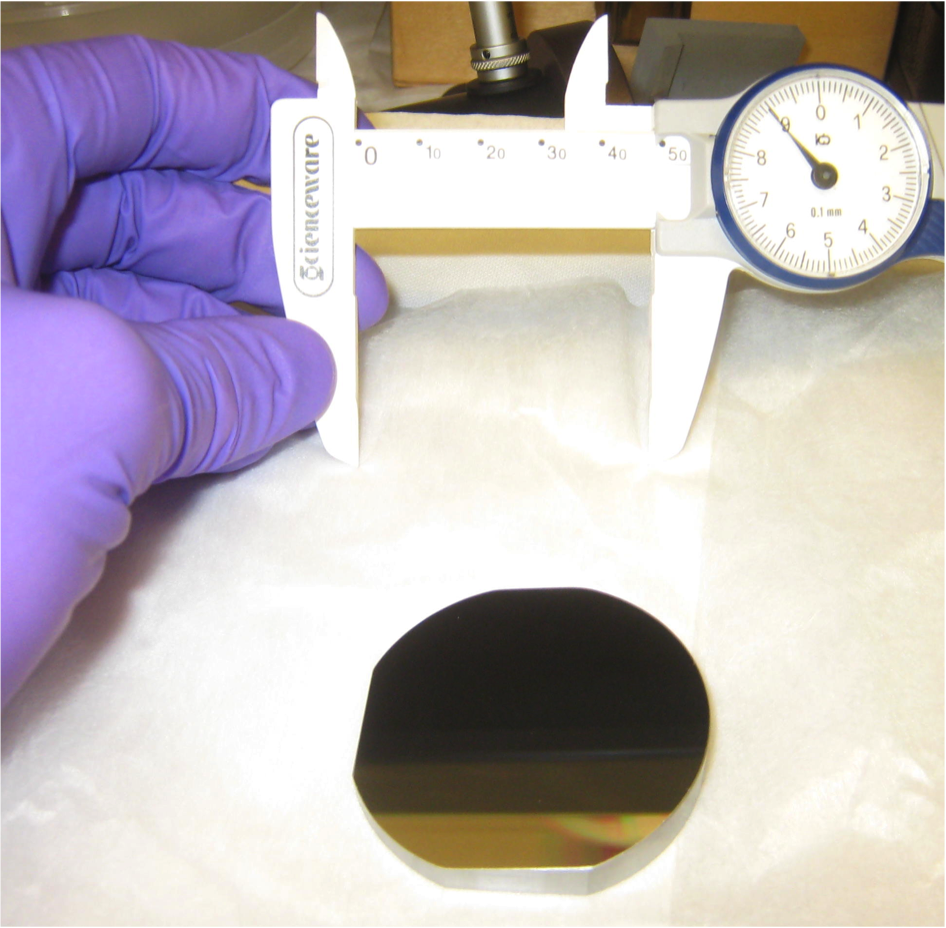
\includegraphics[height=9cm]{A6K_scale.png}
   \end{tabular}
   \end{center}
   \caption[JWST grism [pictures] 
   { \label{fig:im1} 
Photograph of flight grism ``A6K" for JWST-NIRCam.  The outer diameter is 48 mm and the part has an optically usable diameter of 42 mm.  The forward-facing surface has grooves with a period of 15.36 $\mu$m.  The opposite surface has been polished optically flat.  The flats along the perimeter serve as mounting and orientation surfaces}
   \end{figure} 

\subsection{Surface Flatness}
Because the parts are physically larger than the optically active area, it was possible to polish the flat surfaces of the JWST grisms to very high accuracy.  The specification for the polishing vendor was that the surface be flat to $\lambda$/10 peak to valley at 633 nm.  At 3.7 $\mu$m, this specification corresponds to a flatness of ~$\lambda$/60.  The difference of 2.4 in the refractive indices inside and outside the grism imposes similar flatness criteria for a silicon transmission optic to those one would impose on a mirror.  The achieved flatness of the entrance faces (Figure 2) did not always meet this optical specification but, in all cases, was very much better than required for diffraction-limited performance and these faces do not contribute to loss of performance in either throughput or resolution.  


   \begin{figure}
   \begin{center}
   \begin{tabular}{c}
   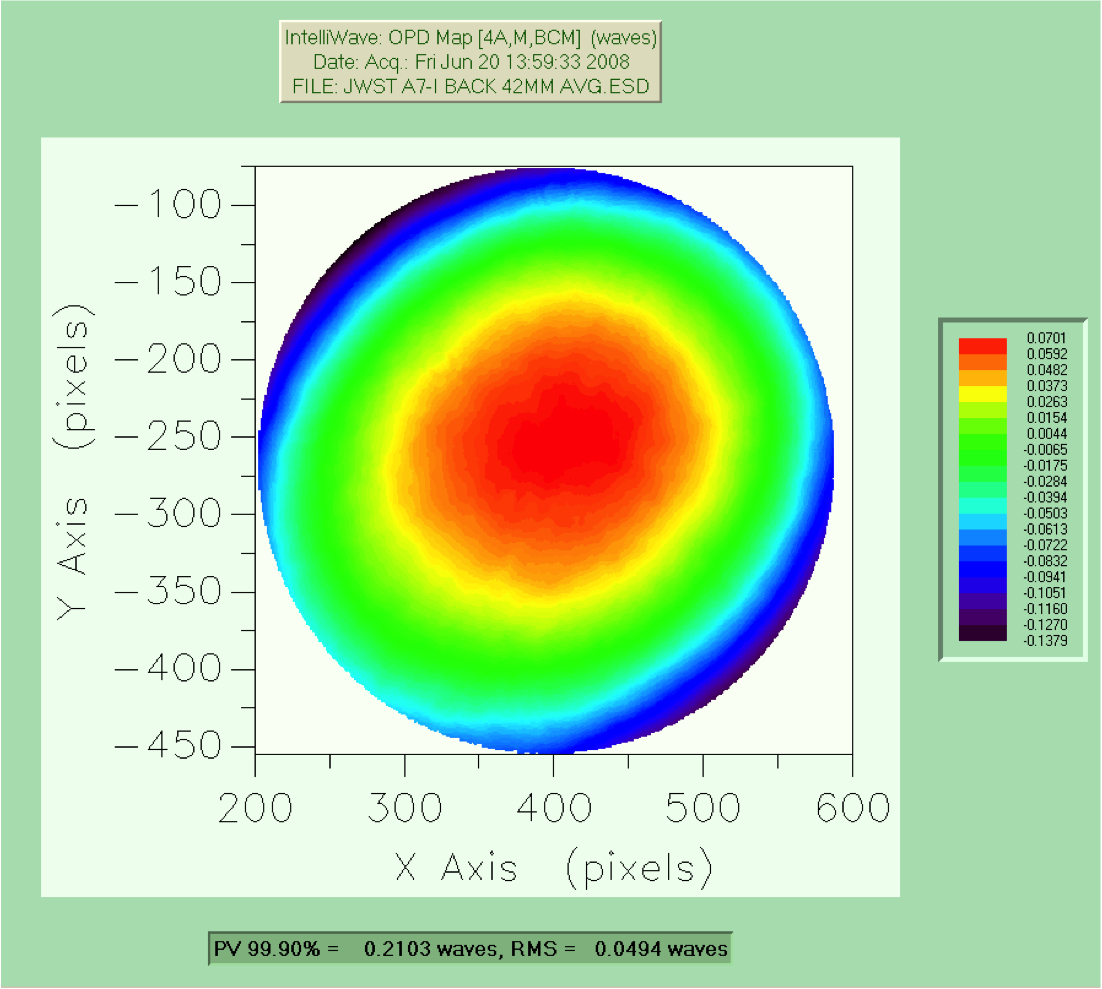
\includegraphics[height=7cm]{A7I_entrance_uncoat.png}
   \end{tabular}
   \end{center}
   \caption[A7-I interferogram] {\label{fig:im2}  Interferogram of the polished entrance surface of JWST trial grism ``A7-I".  The interferogram was taken prior to the application of an antireflection coating. }
   \end{figure} 

\subsection{Groove Geometry}
We form the grooves in the monolithic substrates from which we fabricate the grisms by taking advantage of the significantly different rates at which certain chemicals etch through the different planes in crystalline structure\cite{Marsh07, Tsang1975}.  In our process a solution of KOH etches approximately 60 times faster across the 100 plane than across the 111 plane and a suitably oriented mask of stripes will form triangular grooves at the intersection of 111 planes.  The intersecting planes form an angle of $71\,^{\circ}{\rm}$.  For blaze angles greater than $8\,^{\circ}{\rm}$, this acute angle will result in shadowing of one groove by another in transmission with the amount of shadowing a function of the blaze angle (see Figure 6 of Mar et al. (2006)\cite{Mar06}).  For small prism opening angles, it is not the acute groove vertex but rather the small dams along the grating surface that lead to groove filling factors less than one.  We need the dams to serve as etch stops between the grooves.  For the JWST gratings, the grating constant was 15.36 $\mu$m and the final dam width was about 1.5 $\mu$m.  At the $6.16 \,^{\circ}{\rm}$ opening angle of the JWST prisms, the dams are responsible for the filling factor loss.  The geometric blockage whether by the dams or by the lip of the neighboring acute groove leads to loss in two ways:  direct blockage of the light and, via Babinet's principle, diffraction of an equal amount of light into unwanted orders.  For the geometric blockage of $\sim10\%$ in the JWST grisms, the maximum theoretical transmission is then 0.81.  

\subsection{Microscopic Surface Roughness}
While the etching process results in remarkably flat grooves, point defects in the structure of the crystalline silicon grating substrates can lead to local pits and hillocks, that is, to roughness on various scales, as the anisotropic etching produces the blazed grooves.  The consequences of this roughness are difficult to measure directly as the scattered light produced as a result of it is generally on large angular scales with low peak amplitudes.  Instead, the best ways to evaluate this possible loss mechanism is to examine the roughness of the surfaces directly.  We have done this for an earlier set of grating surfaces using atomic force microscopy\cite{Marsh07} and concluded that the integrated diffuse scattered light due to small-scale roughness is 0.005\% for a Si grism in operation at 3.7$\mu$m.  We have also used interferometric metrology of roughness within individual grooves in the more demanding context of immersion grating production (see Wang et al. in this volume\cite{Wang10}) and find that the loss should be about 0.006\%  if such surfaces are used in transmission.


\subsection{Fresnel Losses}
The large refractive index ($\sim 3.41$ in the near-IR) that gives silicon grisms their large etendue also condemns them to substantial reflective (Fresnel) losses at the vacuum/Si interface.  For uncoated silicon, this loss is $\sim 30\%$ per surface.  When this loss is combined with the geometric loss, the maximum efficiency in the blaze order should be $\sim 0.41$.  Figure 3 shows the transmission versus wavelength curve for one of the NIRCam flight parts.  The tight delivery schedule for these parts did not allow us to measure the performance in first order, where the parts will be used in flight, but the on-blaze transmission of the uncoated gratings in modestly higher orders should be similar.  The peak transmission in 3$^{rd}$ order is 43\%, consistent to within the errors with the theoretical maximum. Even without an antireflection coating, the transmission of this grism is within the low end of the range of published efficiencies for near-IR grisms made from other materials and currently in use at ground-based telescopes, for example NSFCAM's KRS5 grism\cite{Rayner98} demonstrated  efficiencies of 55\%, 50\%, 40\% in orders 2, 3, and 4 which correspond to roughly the L, K, and H near-IR atmospheric bands.  

%Figure 3
   \begin{figure}
   \begin{center}
   \begin{tabular}{c}
   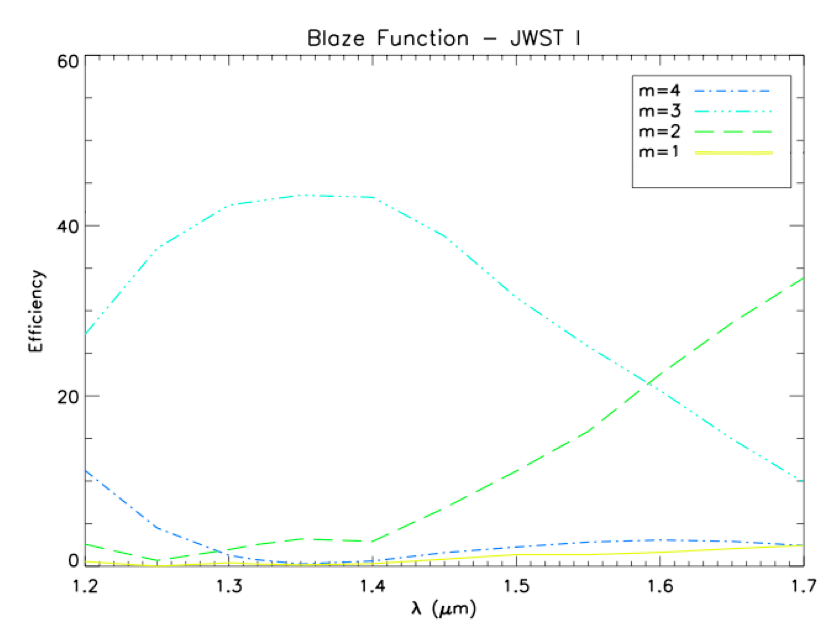
\includegraphics[height=9cm]{A6I_transmission_nt2}
   \end{tabular}
   \end{center}
   \caption[JWST grism transmission] {\label{fig:im3}  Measurement of throughput as a function of wavelength for JWST flight part ``A6-I".  The combination of the geometric blockage by the groove dams and the Fresnel losses results in a theoretical maximum efficiency of $\sim 0.41$ on the blaze.  The plot shows the power in the fifth order and in adjacent orders.} 
   \end{figure} 

\section{Results of Anti-Reflection Coating}
The initial plan for the JWST grisms was to coat only the flat side of each grism with a broad-band antireflection (AR) coating.  An ideal coating on this single face would result in a transmission of 0.57, a performance at the high end of the range of throughputs cited for grisms currently in use.  Figure 4 shows the transmission of a thin silicon wafer witness with an AR coating applied to one air-Si interface.  In the range of 2-5 $\mu$m, the transmission curve is consistent with Fresnel losses from only the uncoated surface, or in other words the AR coating transmits almost 100\% of the incident light.  

In a diffraction limited system, however,  one needs to be concerned about whether the process control for a multilayer coating is sufficiently good to preserve the observed flatness of the entrance face.  We were able to take interferograms of a geometrically similar test piece before and after a broad-band 2-5 $\mu$m antirection coating was applied.  The large-scale phase coherence won in the polishing of this surface has not been degraded by the addition of the multi-layer dielectric AR coating.
   
   %Figure 4
   \begin{figure}
   \begin{center}
   \begin{tabular}{c}
   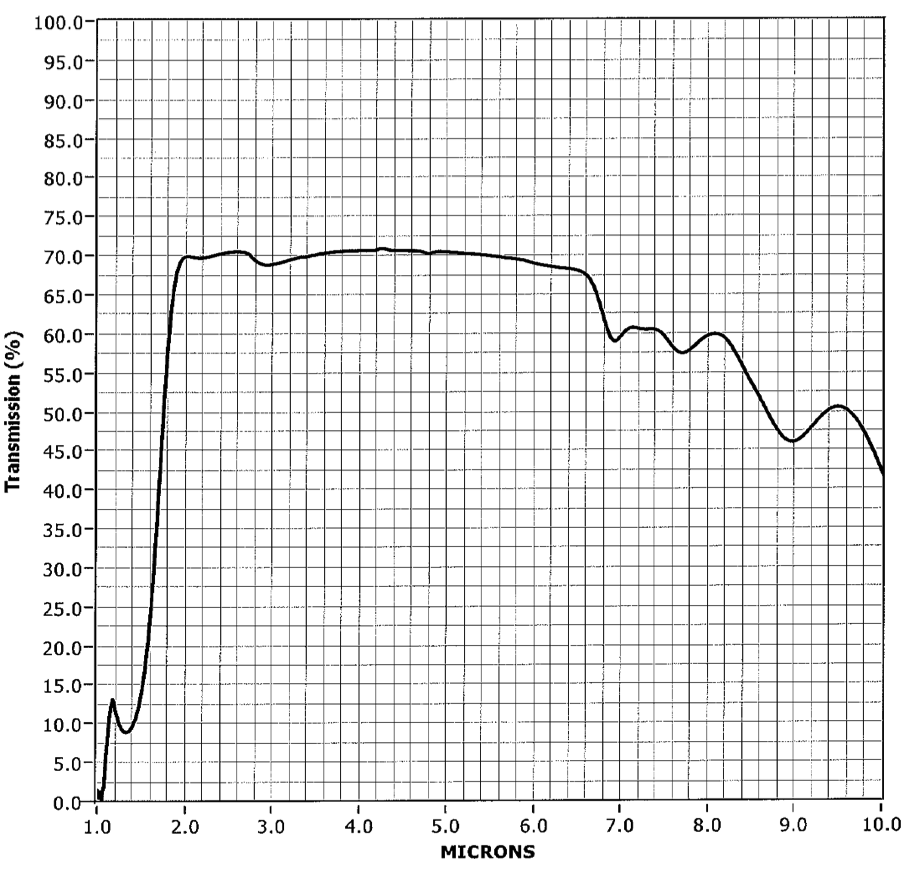
\includegraphics[height=10cm]{ARcoat_trans_siww}
   \end{tabular}
   \end{center}
   \caption[Transmission of single side AR coated silicon wafer witness] {\label{fig:im4}  IR transmission of an optically flat thin silicon wafer witness that was AR coated on a single side.  The wafer does not have grooves on it, and therefore does not have geometric losses.  Since the uncoated air-Si interface suffers 30\% Fresnel loss, the AR coated interface must exhibit close to 100\% transmission between 2 and 5 $\mu$m.  The AR coating is ineffective shortward of 2 $\mu$m, and Si does not transmit short of 1.15$\mu$m.  Figure courtesy of II-VI Inc.} 
   \end{figure} 
 
The only way to improve the delivered throughput beyond that achieved with the single-side coating would be to coat the grism grooves as well with a broad-band AR coating.  Such a procedure faces three potential problems:  (1) The shape of the groove makes it hard to deposit even layers of controlled thickness that are the basis for the efficacy of any antireflection coating. (2) Even small-amplitude variations in the summed thickness of the coatings could diminish the superlative phase coherence of the grating on large scales. (3) Even if the coating preserves coherence on large scales, variations in the deposition thickness within each groove could produce a change in the blaze shape from perfectly flat to structured in a way that might divert power out of the blaze order.

In the course of the development work for the JWST grisms, we were able to test the viability of AR coatings on the grating grooves by putting test coatings onto a prototype.  This prototype ``trial'' part (``A7-I") had the same groove constant and same vertex angle as the flight parts and flight spares but has an $11\,^{\circ}{\rm}$ blaze angle, rather than the $5.75\,^{\circ}{\rm}$ angle shared by the other parts.  The trial part functions well in the mid-infrared but differs from the flight parts in having its second-order rather than first-order blaze peak at the center of the band for the JWST long wavelength camera.  The difference in the prism opening angle and groove blaze angle means that the wavelength at the peak of the blaze is not undeviated as it is for the flight parts.  We coated this part with the same antireflection coating used for the flat surfaces of the flight parts, coating it first on the flat side and then, after measurement, on the grooved surfaces as well.  Throughput measurements were carried out by our group at UT Austin with a scanning monochromator or by II-VI Infrared Inc with their spectrophotometer.  The UT measurements were performed by measuring the ratio of the transmitted signal strength at the appropriate angle for the second-order beam to the signal from the monochromator incident on the detector with no intervening dispersive element.

%Figure 5: a) Transmission of uncoated trial part
                 %b) Transmission of coated trial part
   \begin{figure}
   \begin{minipage}[b]{0.5\linewidth} % A minipage that covers half the page
   \begin{tabular}{c}
   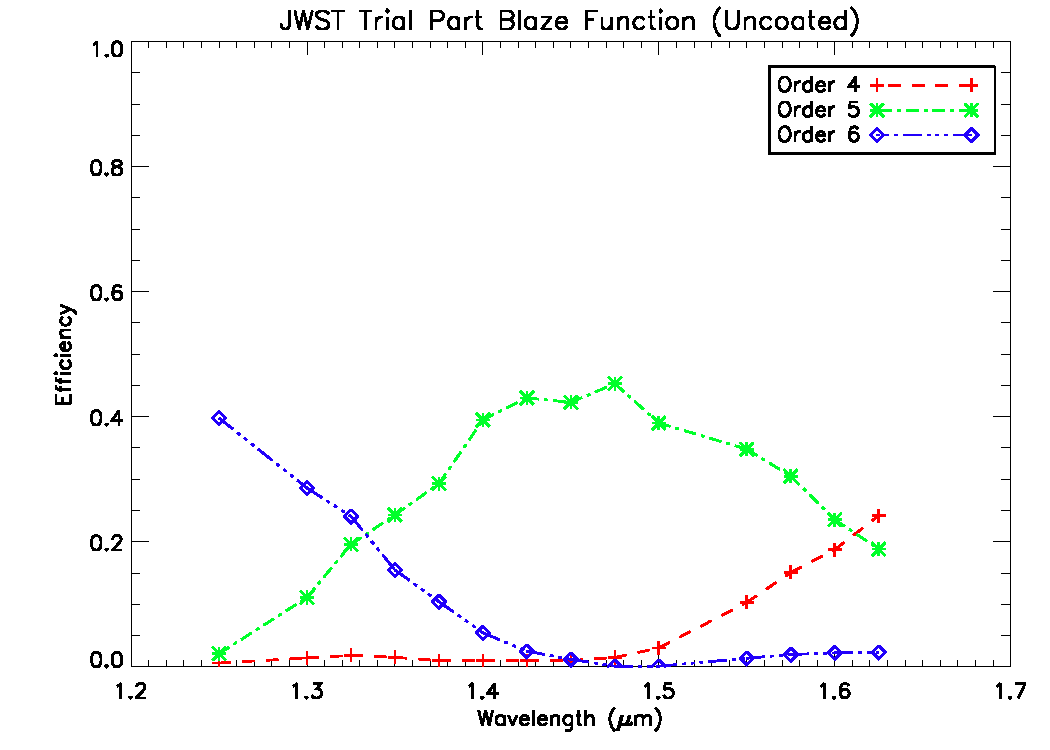
\includegraphics[width=\textwidth]{A7I_uncoated_trans.pdf}
   \end{tabular}
   \end{minipage}
   \hspace{0.01cm} % To get a little bit of space between the figures
\begin{minipage}[b]{0.5\linewidth}
   \begin{tabular}{c}
   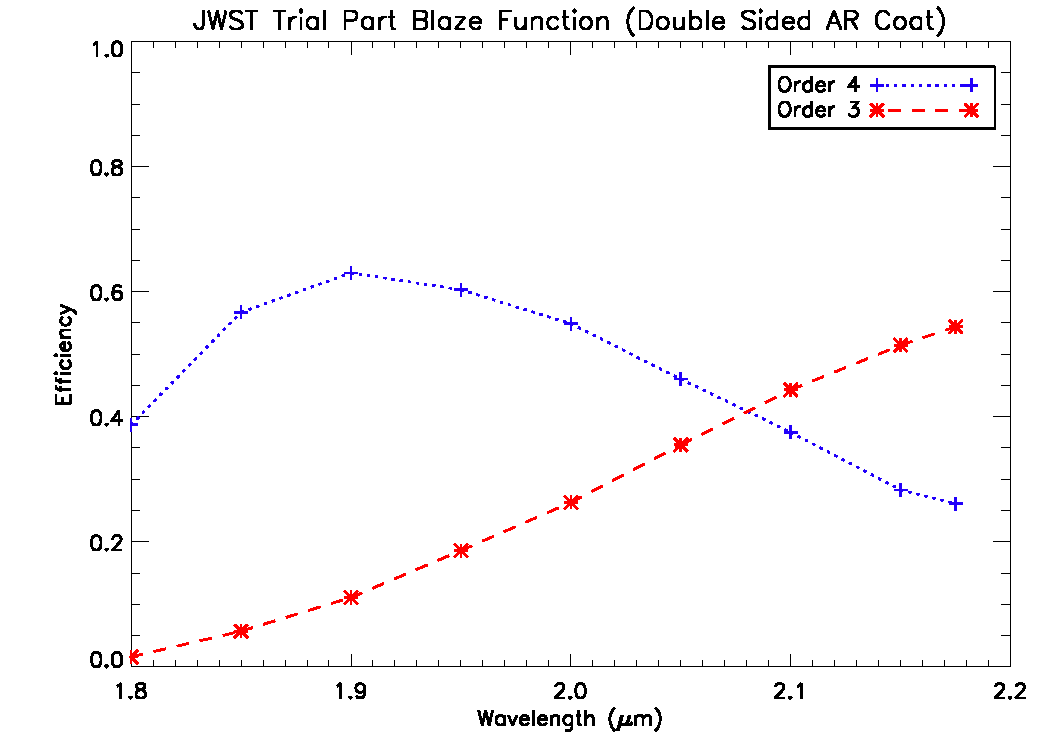
\includegraphics[width=\textwidth]{A7I_coated_2.pdf}
   \end{tabular}
   \end{minipage}
   \caption[JWST grism transmission] {\label{fig:im5}  Transmission of trial part A7-I.  The interferograms were taken with the surfaces (left) uncoated and (right) coated on both entrance and grating surfaces.  The ineffectiveness of the AR coating shortward of 2.0 $\mu$m (cf. Figure 4) stifled a direct comparison of transmission at the same wavelengths before and after coating.  The poor transmission below 2.0 $\mu$m is apparent in the right panel, since the $4^{th}$ order curve is suppressed before it reaches its blaze peak near 1.8 $\mu$m.  A similar measurement at 3.1-4.0 $\mu$m shows 75\% peak efficiency for the double-side coated grism.}
   \end{figure} 

The left panel of Figure 5 shows the performance of this part prior to the application of the coating while the right panel shows the transmission after A7-I had been AR coated on both its entrance and exit surfaces.  The right panel of Figure 5 does not reveal the peak on-blaze efficiency for two reasons- (1) the narrow wavelength range can only capture the $4^{th}$ order blaze peak and (2) the AR coating is ineffective at wavelengths shorter than 2.0 $\mu$m, suppressing the peak near 1.8 $\mu$m.  A coarse estimate for the blaze efficiency can be obtained by summing the power in orders 3 and 4 at a given wavelength, yielding an expected value for the peak efficiency of 80\%, which would be consistent with the maximum 81\% permitted by geometrical losses.  Our group has also performed throughput measurements from 3.1 to 4.0 $\mu$m that indicate 75\% efficiency at the $2^{nd}$ order blaze peak at 3.7 $\mu$m (see figure in C. Deen et al. in preparation).  The measurements at $2^{nd}$ order also indicate negligible power in the adjacent orders at 3.7 $\mu$m.  This observation is important because it means power was not diverted out of the blaze order after the AR coating was applied.  The multi-layer coating must not have altered the shape of individual grooves- variations in the deposition thickness within each groove must be very small.  This claim is also weakly supported by pre- and post- coating optical reflection measurements, which show similar ratios of power in the first and second brightest orders at 633 nm.  

Figure 6 shows a comparison of the 633 nm Littrow interferogram of the grooved surface of the trial part before (left) and after (right) the application of the antireflection coating.  While the images themselves appear quite dissimilar, the numbers at the bottom of the plot tell the true story.  The peak to valley deviation in the reflected phase front is virtually identical in the two cases and is extremely small ($< \lambda/100$ at the blaze wavelength). 



%Figure 6: a) Interferometry of uncoated trial part 31mm
                 %b) Interferometry of coated trial part 31mm
   \begin{figure}
   \begin{minipage}[b]{0.5\linewidth} % A minipage that covers half the page
   \begin{center}
   \begin{tabular}{c}
   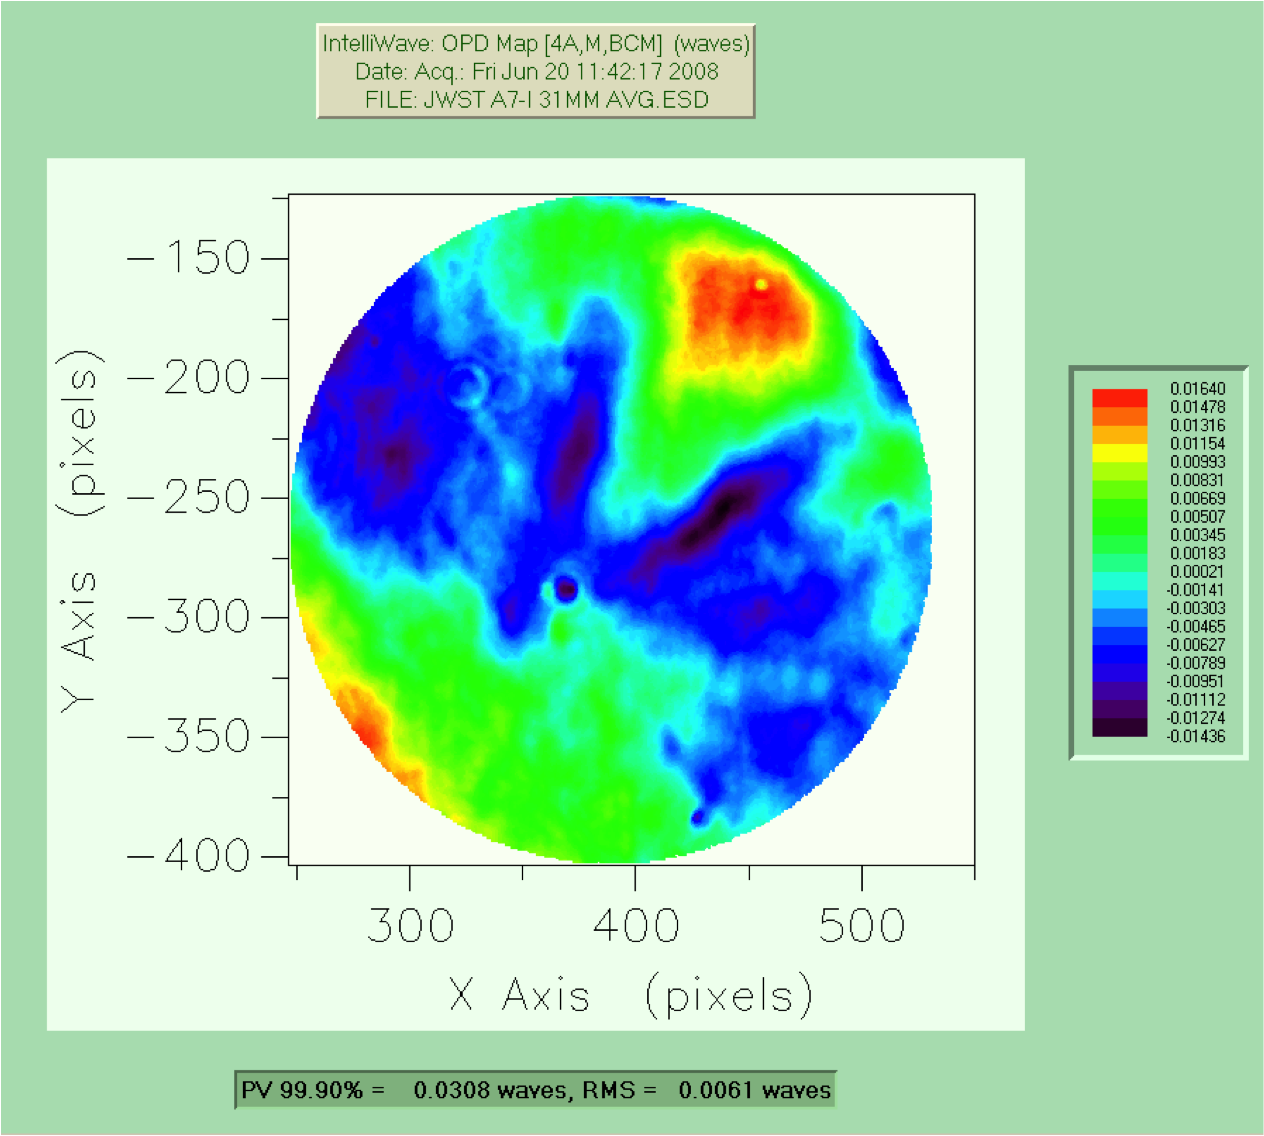
\includegraphics[width=\textwidth]{A7I_interf_31mm_grat_uncoat.png}
   \end{tabular}
   \end{center}
   \end{minipage}
   \hspace{0.0001cm} % To get a little bit of space between the figures
\begin{minipage}[b]{0.5\linewidth}
\begin{center}
   \begin{tabular}{c}
   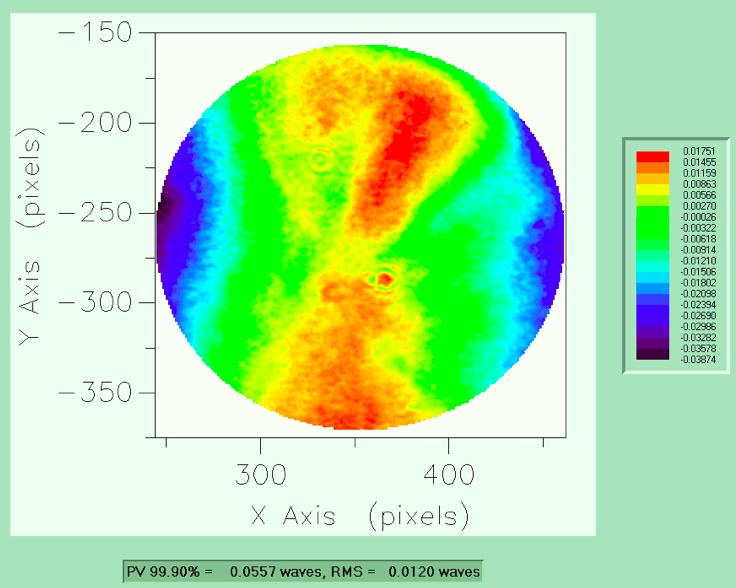
\includegraphics[width=\textwidth]{A7I_post_coat.png}
   \end{tabular}
   \end{center}
   \end{minipage}
   \caption[Trial part groove interferogram] {\label{fig:im6}  Optical interferograms at 633nm of the central 31 mm of the grooved surfaces of the trial part, A7-I.  The left figure shows the grooved surface before AR coating.  On the right is the interferogram of the grating surface after AR coating.  The RMS and peak to valley wavefront errors are printed at the bottom of the figures- \em{before}\em: PV- 0.0308, RMS- 0.0061 waves; \em{after}\em: PV- 0.0557, RMS- 0.0120 waves.}
   \end{figure} 


\section{Conclusions}
In summary, we have completed a set of six high performance silicon grisms for the NIRCam instrument on JWST.  The grisms are produced with precision photolithography and anisotropically etching the Si crystal plane.  By enumerating the loss mechanisms we saw that geometric and Fresnel losses limit the throughput of silicon grisms to about 41\%.  When the entrance and grating surfaces are coated with a broad band anti-reflection coating, Fresnel losses become negligibly small.  Measurements of a sample double side AR coated grism indicate on blaze throughput of about 75\%, marginally below the 81\% expected for purely geometric losses.  The grating performance was not significantly degraded by the multi-layer dielectric coating, as evinced by interferometry and optical reflection efficiency measurements.
